\subsection{Análise de Resposta com Controlador Proporcional e PID Ajustado}

Esta seção compara a resposta do sistema utilizando um controlador proporcional e um controlador PID ajustado, especificamente configurados com os parâmetros \( K_p = 8.958 \), \( K_i = 0.310 \), e \( K_d = 0.805 \). A análise foca na eficácia de cada controlador em atingir e manter o valor de referência desejado, sob uma amplitude de degrau de \( A = 2.5 \). Este estudo visa elucidar as vantagens e limitações de cada abordagem de controle em termos de resposta dinâmica e estabilidade.

\begin{figure}[H]
    \centering
    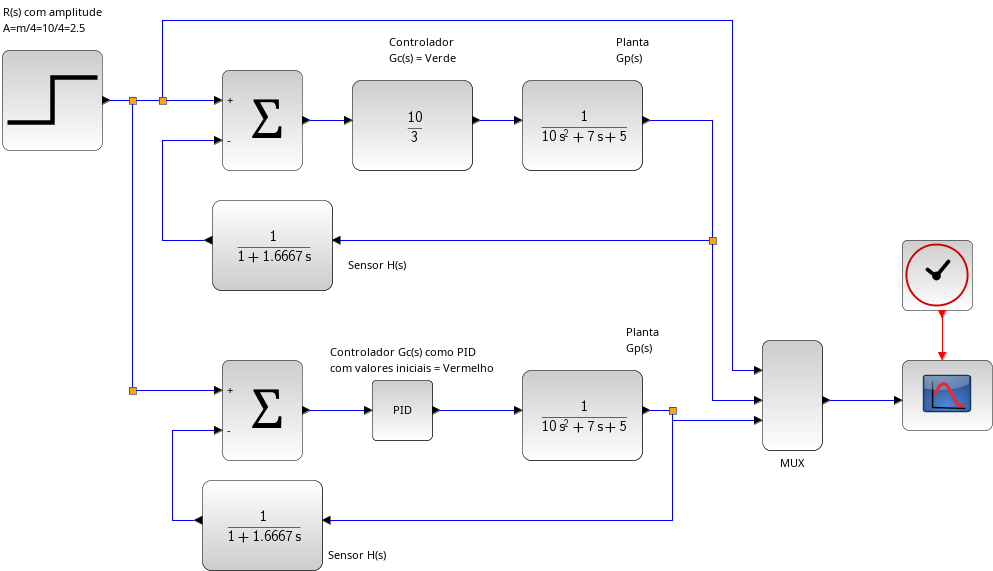
\includegraphics[width=0.8\textwidth]{6-atividade/assets/b/diagrama-comparacao-proporcional-pid.png}
    \caption{Diagrama ilustrativo do sistema de controle comparando a resposta com controlador proporcional e PID ajustado.}
    \label{fig:diagrama-comparacao-proporcional-pid}
\end{figure}

\begin{figure}[H]
    \centering
    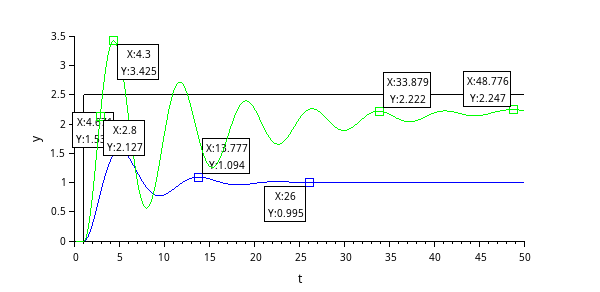
\includegraphics[width=0.8\textwidth]{6-atividade/assets/b/comparacao-proporcional-pid.png}
    \caption{Resposta temporal do sistema com controlador proporcional e PID ajustado.}
    \label{fig:comparacao-proporcional-pid}
\end{figure}

\subsubsection{Controlador Proporcional (Cor Azul)}
\textbf{Comportamento:}
O controlador proporcional oferece uma resposta imediata, característica desejada em muitas aplicações industriais por sua simplicidade e eficácia em sistemas menos complexos. No entanto, como evidenciado na Figura \ref{fig:comparacao-proporcional-pid}, ele falha em eliminar o erro de estado estacionário, estabilizando abaixo do valor de referência desejado.

\textbf{Estado Estacionário:}
A incapacidade de ajustar o erro estacionário torna o controlador proporcional menos adequado para aplicações que demandam precisão contínua e ajuste fino, pois não pode corrigir desvios permanentes sem intervenção externa.

\subsubsection{Controlador PID Ajustado (Cor Verde)}
\textbf{Comportamento:}
A configuração ajustada do PID demonstra superioridade em alcançar e manter o valor desejado rapidamente, com uma oscilação inicial (overshoot) significativamente reduzida e rápida estabilização, como ilustrado na Figura \ref{fig:comparacao-proporcional-pid}. Essa resposta é crucial em processos que não podem tolerar grandes desvios temporários ou onde o controle preciso é crítico.

\textbf{Estado Estacionário:}
O controlador PID, ajustado com parâmetros otimizados, mantém o valor de referência com alta precisão, ilustrando a importância da ação integral em corrigir erros acumulados e a ação derivativa em antecipar e mitigar futuras variações, resultando em uma resposta estável e precisa.

\subsubsection{Conclusão}
A análise comparativa entre o controlador proporcional e o PID ajustado destaca a simplicidade e a resposta imediata do primeiro, ideal para aplicações menos críticas, contra a precisão e a estabilidade superior do segundo. Com parâmetros ajustados (\(K_p = 8.958\), \(K_i = 0.310462589\), \(K_d = 0.80525\)), o controlador PID se adapta melhor às necessidades de aplicações que exigem controle dinâmico e alta fidelidade.

No entanto, é crucial reconhecer que os ajustes nos parâmetros \(K_p\), \(K_i\), e \(K_d\) do PID não são sem riscos e devem ser continuamente revisados. Alterações imprudentes em \(K_p\) podem levar a overshoots excessivos e instabilidade, enquanto \(K_i\) elevado pode causar oscilações indesejadas e resposta lenta, afetando negativamente a eficácia do sistema. Ajustes em \(K_d\) também requerem cautela, pois, embora possam melhorar a estabilidade, podem resultar em uma resposta demasiadamente amortecida.

Portanto, é recomendado que os ajustes nos parâmetros do PID sejam feitos com base em testes rigorosos e análise cuidadosa. A busca por um equilíbrio ótimo entre rapidez de resposta, estabilidade e precisão deve ser uma prática regular, adaptando o controlador às variações nas condições operacionais e às exigências específicas de cada aplicação. Esse processo contínuo de otimização ajuda a assegurar a performance aprimorada e a segurança do sistema controlado.
